\documentclass{article}

\usepackage{graphicx}
\usepackage{indentfirst}
\usepackage[a4paper, total={6in, 8in}]{geometry}
\usepackage{hyperref}
\usepackage{fancyhdr}
\usepackage{xepersian}
\settextfont{[XB Zar.ttf]}
\setlatintextfont{[Times New Roman.ttf]}

\begin{document}


%title page%
\begin{titlepage}
	\begin{center}
		\vspace{0.2cm}
		
		
\includegraphics[width=0.4\textwidth]{sharif.png}\\
		\vspace{0.2cm}
		\textbf{ \Huge{آزمایش شماره 8}}\\
		\vspace{0.25cm}
		\textbf{ \Large{آز شبکه - دکتر بردیا صفایی}}
		\vspace{0.2cm}
		
		
		\large \textbf{دانشکده مهندسی کامپیوتر}\\\vspace{0.1cm}
		\large   دانشگاه صنعتی شریف\\\vspace{0.2cm}
		\large   ﻧﯿﻢ‌سال اول ۰۱-۰۲ \\\vspace{0.10cm}
		\large{ گروه 8:}\\
		\large{\href{mailto:mehrshad.mirmohammadi@gmail.com}{مهرشاد میرمحمدی - 98109634}}\\
		\large{\href{mailto:parhaamsaremi@gmail.com}{پرهام صارمی - 97101959}}\\
		\large{\href{mailto:mofayezi.m@gmail.com}{محمدرضا مفیضی - 98106059}}\\
	\end{center}
\end{titlepage}
%title page%

\newpage

%pages header
\pagestyle{fancy}
\fancyhf{}
\fancyfoot{}
\setlength{\headheight}{59pt}
\cfoot{\thepage}
\lhead{آزمایش شماره 8}
\rhead{
\includegraphics[width=0.1\textwidth]{sharif.png}\\
		دانشکده مهندسی کامپیوتر
}
\chead{آز شبکه - گروه ۸}
%pages header


ابتدا در محیط \lr{packet tracer} سناریو گفته شده در کلاس را طراحی می‌کنیم (شکل \ref{fig:scenario-1}).
ما آدرس‌ها را دقیقا همانند ویدیو کلاس قرار داده‌ایم.
\begin{figure}[h!]
	\centering
	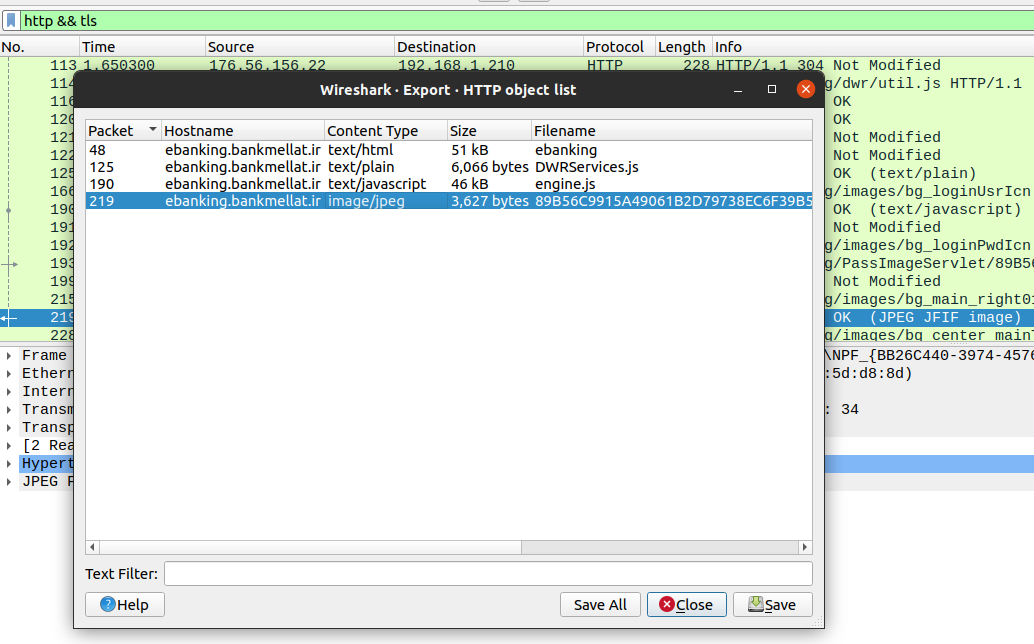
\includegraphics[width=0.6\columnwidth]{1.png}
	\caption{تصویر پیاده‌سازی سناریو در محیط \lr{packet tracer}}
	\label{fig:scenario-1}
\end{figure}

سپس بر روی سرور، سرویس DHCP را فعال کرده و تنظیمات لازم را انجام می‌دهیم.
(شکل \ref{fig:scenario-2})

\begin{figure}[h!]
	\centering
	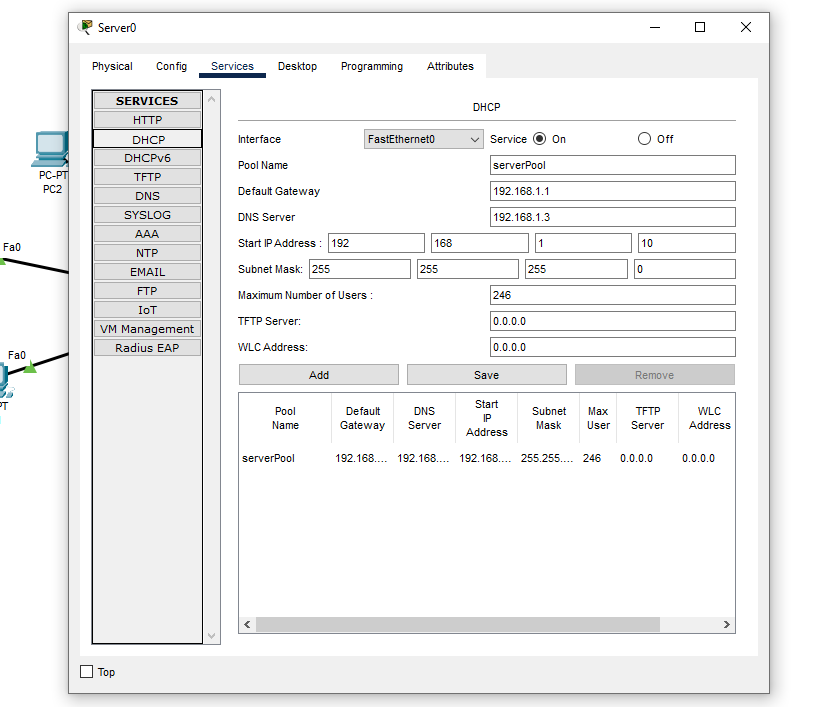
\includegraphics[width=0.6\columnwidth]{2.png}
	\caption{تنظیمات سرویس DHCP بر روی سرور}
	\label{fig:scenario-2}
\end{figure}

بعد از آن، با یکی از PC ها چک می‌کنیم که گرفتن IP با استفاده از سرویس DHCP به درستی انجام شود(شکل \ref{fig:scenario-3}).

\begin{figure}[h!]
	\centering
	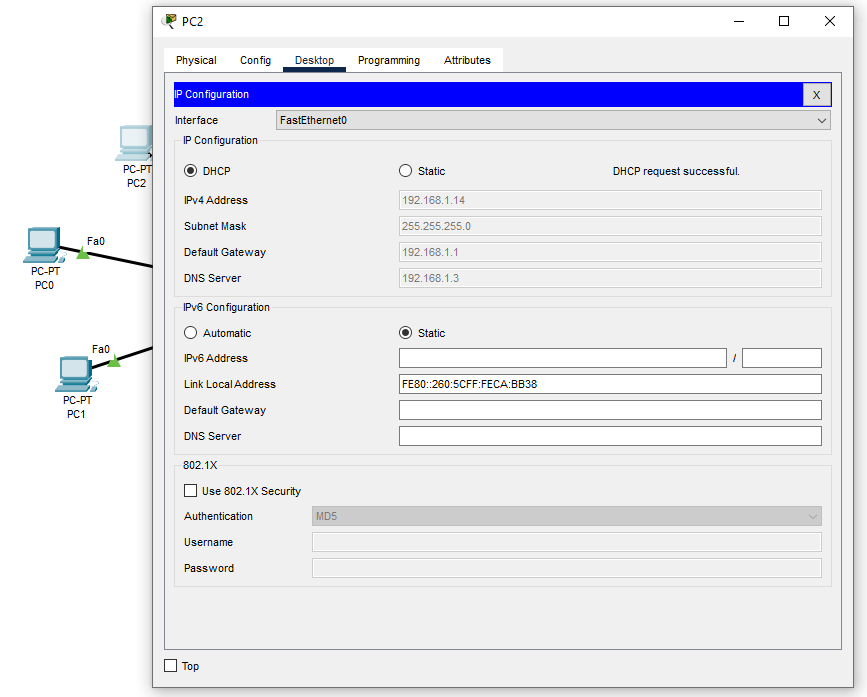
\includegraphics[width=0.6\columnwidth]{3.png}
	\caption{بررسی درستی گرفتن IP توسط یکی از PCها.}
	\label{fig:scenario-3}
\end{figure}

اکنون به تنظیم \lr{DHCP Snooping} می‌پردازیم. برای این کار اول IP های گرفته شده توسط هر PC رو آزاد می‌کنیم. برای این کار از دستور شکل \ref{fig:scenario-4} استفاده می‌کنیم. این کار را برای تک تک PC ها انجام می‌دهیم.

\begin{figure}[h!]
	\centering
	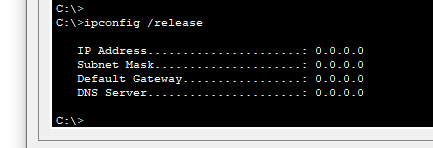
\includegraphics[width=0.6\columnwidth]{4.png}
	\caption{آزاد کردن IP گرفته شد در هر PC}
	\label{fig:scenario-4}
\end{figure}

سپس قابلیت \lr{DHCP Snooping} را فعال می‌کنیم. می‌توان دید که هنوز VLAN ای برای این ابزار مشخص نشده‌است(شکل \ref{fig:scenario-5}).

\begin{figure}[h!]
	\centering
	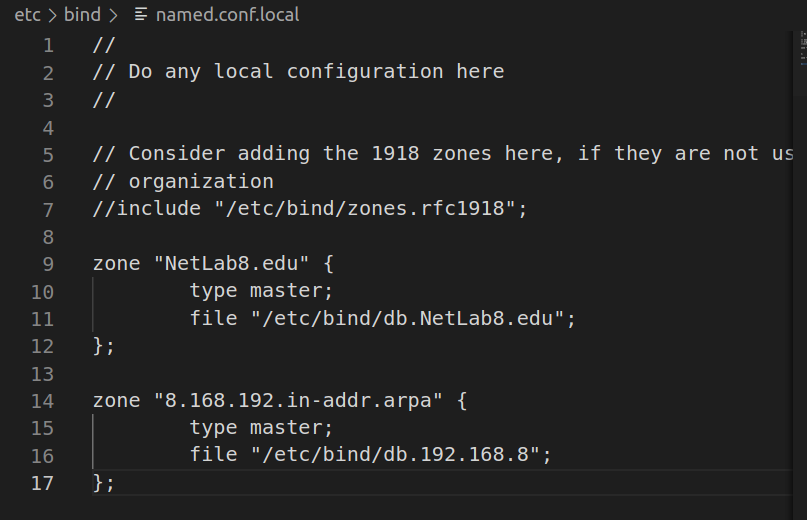
\includegraphics[width=0.6\columnwidth]{5.png}
	\caption{فعلا سازی قابلیت \lr{DHCP Snooping}}
	\label{fig:scenario-5}
\end{figure}

در گام بعد VLAN مناسب را مشخص می‌کنیم (شکل \ref{fig:scenario-6}).


\begin{figure}[h!]
	\centering
	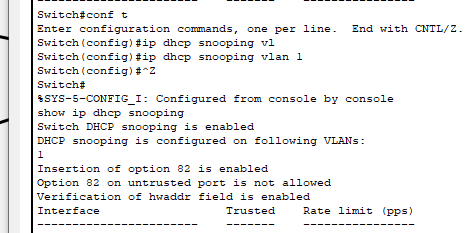
\includegraphics[width=0.6\columnwidth]{5.1.png}
	\caption{اضافه \lr{VLAN 1} به \lr{DHCP Snooping}}
	\label{fig:scenario-6}
\end{figure}

اکنون می‌توان دید امکان گرفتن IP توسط DHCP وجود ندارد (شکل \ref{fig:scenario-8}). دلیل آن هم این است که هنوز port ای را مورد اعتماد قرار نداده‌ایم.

\begin{figure}[h!]
	\centering
	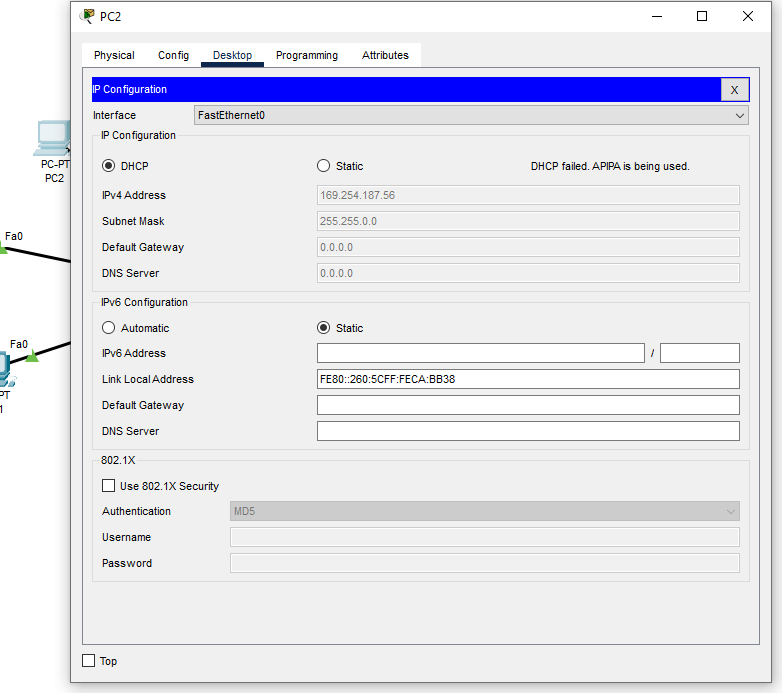
\includegraphics[width=0.6\columnwidth]{6.png}
	\caption{ناتوانی در گرفتن IP زمانی که هنوز interface‌ ای را مورد اعتماد قرار نداده‌ایم}
	\label{fig:scenario-8}
\end{figure}

بعد از آن پورت \lr{fastEthernet 0/1} که پورت‌ای هست که به سرور متصل است را مورد اعتماد می‌کنیم (شکل \ref{fig:scenario-7}).

\begin{figure}[h!]
	\centering
	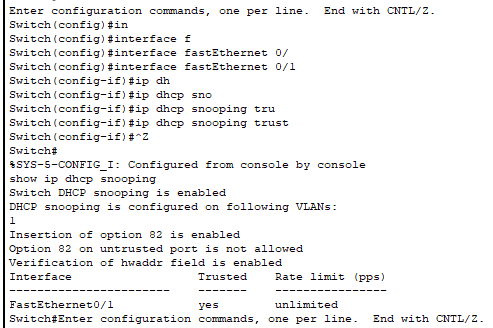
\includegraphics[width=0.6\columnwidth]{5.2.png}
	\caption{مشخص کردن \lr{fastEthernet 0/1} به عنوان قابل اعتماد}
	\label{fig:scenario-7}
\end{figure}

حال عملیات گرفتن IP در PC ها با موفقیت انجام می‌شود (شکل \ref{fig:scenario-10}).

\begin{figure}[h!]
	\centering
	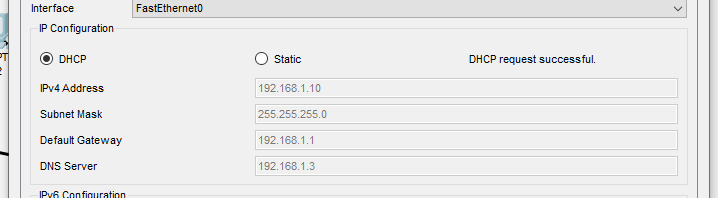
\includegraphics[width=0.6\columnwidth]{8.png}
	\caption{موفقیت در گرفتن IP بعد از اعتماد‌سازی به port مربوطه}
	\label{fig:scenario-10}
\end{figure}

در نهایت می‌توان پایگاه‌داده‌ی ذخیره‌ شده در داخل سوییچ را مشاهده کرد که به ما تناظر بین هر IP و port را می‌دهد (شکل \ref{fig:scenario-9}). این پایگاه داده برای ملاحظات امنیتی دیگر سودمند است.

\begin{figure}[h!]
	\centering
	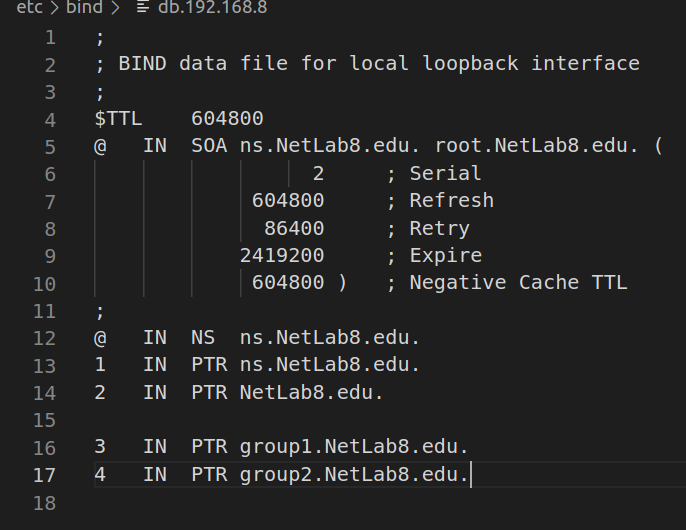
\includegraphics[width=0.6\columnwidth]{7.png}
	\caption{پایگاه داده‌ی ذخیره‌ شده در switch که در آن تناظر بین port ها و IP ها مشخص شده‌اند.}
	\label{fig:scenario-9}
\end{figure}

\end{document}
